\chapter{Analysis of correlated SiPM noise}
\label{ch:anal}

In the previous chapters we studied the sources of noise in the procedure to
identify and measure a single signal. However the photodetector itself produces
pulses which are not due to a detected photon. There are two kinds of these:
pulses which are produced independently of incident light, and pulses which are
produced by another pulse. The latter case is called \emph{correlated noise}.

We will give a brief explanation and classification of the SiPM noise and then
analyze it on a specific tile with LNGS laser data. We will see that we can
reliably measure only the correlated noise, hence the chapter title.

There are two goals in characterizing the SiPM noise. First, a quantitative
model of the noise is needed for the DarkSide20k simulation, and we will
provide an estimate of the parameters for a recent new production of SiPMs.
Second, our ``direct'' analysis method that looks at each single pulse in a
complete recorded finely-sampled waveform provides a cross-check for more
indirect methods that will be employed online in the VETO system which has less
powerful readout electronics.

\marginpar{I should add some reference for charge integration methods. Maybe
the article where I found the Borel the first time, \cite{chmill2017}. I may
do this in the local conclusions.}

\section{Theory}

\marginpar{In chapter~\ref{ch:snr} I will add a qualitative description that
can be deduced from the 2d histogram without previous knowledge apart from the
acquisition setup (the laser position). Just as an epistemic exercise. I must
also add the definition of PE.}

In \autoref{ch:snr} we briefly introduced the Silicon Photomultiplier (SiPM).
We will now give a more detailed explanation, mainly following
\cite[ch.~3]{savarese2018}. For a general introduction to semiconductor
detectors (but not the SiPM), see \cite[ch.~11]{knoll2010}.

The difference between a SiPM and older kinds of semiconductor detectors is
that the SiPM has a binary response: the amplitude of the output is not
proportional to the energy released by the detected particle. In this sense
they are analogous to Photomultiplier Tubes (PMTs), because they are designed
to detect just the presence of a photon with high efficiency ($\sim\SI{50}\%$).

A SiPM is composed by a grid of \emph{cells}. The cells are Single Photon
Avalanche Photodiodes (SPADs). A SPAD is a photodiode operated in reverse bias
above its breakdown voltage in series with a \emph{quenching resistor}. Since
the bias is above breakdown, if a current starts in the photodiode it will be
self sustaining and would normally destroy the diode. The resistor in series
lowers the potential difference on the diode when a current flows through it,
stopping the current because the diode goes below breakdown, so the output
pulse will have duration and amplitude uniquely determined by the resistor and
the capacitance of the diode junction, independently of the initial release of
energy that triggered the current.

The difference between the bias and the breakdown voltage is called
\emph{overvoltage}, and is often indicated with the unit ``\si{VoV}'' meaning
``Volt overvoltage''.

The output from all the cells is summed analogically, so if multiple cells are
triggered simultaneously, the amplitude of the output pulse is discretized and
proportional to the number of fired cells. As we already said in
\autoref{ch:snr}, we will use the term ``PE'', standing for ``photoelectrons'',
as a unit when indicating the number of cells corresponding to a pulse.

\subsection{SiPM noise}

The initial creation of an electron-hole pair that starts the avalanche in the
photodiode can either be caused by an absorbed photon or by a thermal
fluctuation. The latter case happens randomly with fixed probability, and the
resulting rate of random pulses is called \emph{dark count rate}, where
``dark'' stands for the fact that this amounts to the total rate of pulses when
the photodiode is kept isolated from light.

The last sentence is actually not accurate because a ``primary'' pulse, either
a dark count or a photon, by various mechanisms can induce other pulses, that
can themselves recursively produce tertiary pulses in the same way. The four
ways in the proliferation of pulses are (see \autoref{fig:sipmnoise}):

\begin{description}

    \item[Afterpulses] During the avalanche, charge carriers can remain trapped
    into impurities and imperfections of the crystal. They are released
    afterwards at random, starting another avalanche in the same cell.
    
    \item[Direct cross talk (DiCT)] A photon emitted by an avalanche can
    trigger a nearby cell.
    
    \item[Delayed cross talk (DeCT)] Instead of hitting directly another cell,
    the photon can be absorbed in the shared crystal substrate and generate
    a hole that travels up until it passes through a cell and triggers it.
    
    \item[Delayed afterpulse] In the latter case, if the hole hits the
    originating cell, we call it delayed afterpulse instead of DeCT.

\end{description}

\begin{figure}
    
    \centering
    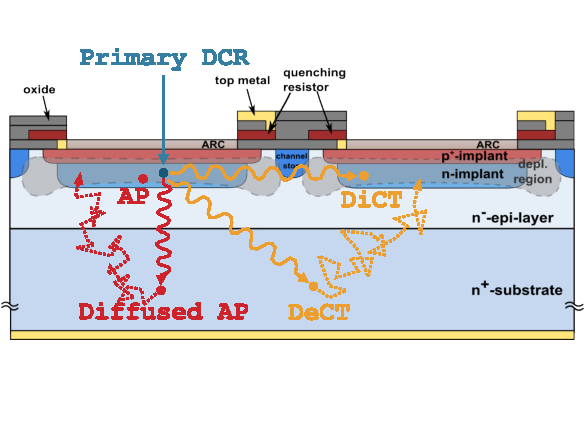
\includegraphics[width=0.85\textwidth]{sipmnoise}
    
    \caption{\label{fig:sipmnoise} Schematic of SiPM noises overlaid on the
    cross section of the device: AP (afterpulse), DiCT (direct cross talk),
    DeCT (delayed cross talk). From \cite[53]{savarese2018}.}
    
\end{figure}

The cells are less than \SI1{mm} wide, so the DiCT pulse starts within \SI1{ps}
of the originating pulse, while as we saw in \autoref{ch:snr} even just the
peak of the pulse lasts $\sim\SI{10}{ns}$. This means that the effect of the
DiCT is multiplying the height of the pulse by an integer factor, because the
overlapping pulses are well aligned. Afterpulses and DeCT, instead, can arrive
with a significative delay, and thus can be distinguished from the originating
pulse.

The reason why we classify separately the delayed pulses, instead of having an
overarching category of ``delayed noise'', is that afterpulses have a different
amplitude. The shape of the pulse is a sharp peak followed by an exponentially
decaying tail. This tail is due to the capacitance of the reverse-biased
junction that recharges through the quenching resistor after being discharged
inside the diode by the avalanche. A pulse generated by the same cell before
the recharge is complete can only use up the charge present in that moment.
Delayed cross talk, instead, has full amplitude because it involves a different
cell. See \autoref{fig:sipmnoiseampl}.

\begin{figure}
    
    \centering
    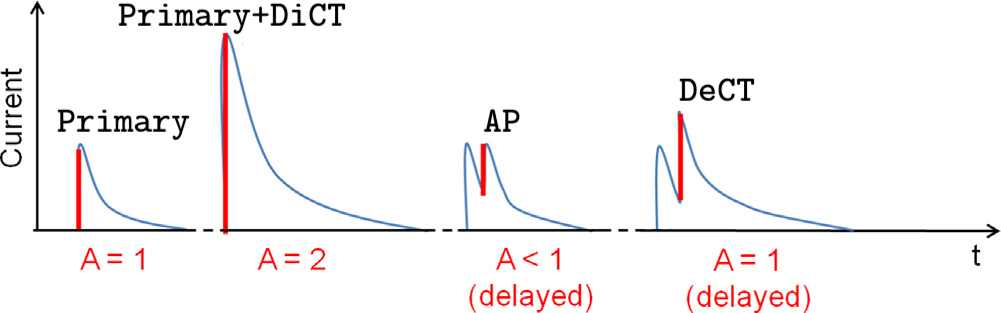
\includegraphics[width=0.85\textwidth]{sipmnoiseampl}
    
    \caption{\label{fig:sipmnoiseampl} Schematic of noise pulses. From
    \cite[4]{nagy2014}.}
    
\end{figure}

\subsection{DiCT model}

As we said, noise pulses can themselves produce other noise pulses as well. We
can imagine quite complicated interactions, for example: a DiCT induces a DeCT
on the original cell, thus producing a ``secondary'' delayed afterpulse. Or a
DiCT induces an afterpulse that induces a DiCT on the originating cell, again
with an afterpulse as final outcome. If the probabilities involved are small
enough, we should get by with the following simplifying assumption: that for
each pulse, the DiCT involves new cells that were not previously involved in
the chain, and the distribution of the number of DiCT at each step is fixed.

For the distribution to use for the generation model of DiCT, we follow
\cite{vinogradov2012}. Even when multiple DiCT steps are chained, the combined
delay is very small compared to the duration of the pulse, so the overall
effect of the complete DiCT ``tree'' is still to multiply the amplitude of the
first pulse. This means that at the end we just need to know the distribution
of the total number of consecutive DiCT.

For the single DiCT step, we consider two distributions: Bernoulli and Poisson.
In the first case we assume that a cell can induce a DiCT in at most just
another cell. In the second, we assume that there is a infinite population of
other cells, each with a fixed probability to be triggered. Clearly these two
cases are ``opposite'' approximations. In the first case, the distribution of
the total number of PE $k$ is Geometric. If $p$ is the probability of
generating a DiCT at each step, the distribution is
%
\begin{equation}
    P_G(k;p) = p^{k-1}(1-p), \quad k \ge 1, \quad p \in [0,1).
    \label{eq:geometric}
\end{equation}
%
Note that the conventional parametrization of the Geometric distribution is
different, with $p$ and $1 - p$ interchanged. We use this formulation because
it is more intuitively comparable with the other case. If the branching
distribution is Poisson with mean $\mu_B$, the total distribution is the Borel,
%
\begin{equation}
    P_B(k;\mu_B) = e^{-k\mu_B} \frac {(k\mu_B)^{k-1}} {k!},
    \quad k \ge 1, \quad \mu_B \in [0,1).
    \label{eq:borel}
\end{equation}
%
If it was $\mu_B \ge 1$, $k$ would diverge with nonzero probability.

The formula for the mean is formally the same for the two distributions,
%
\begin{equation}
    E[k] = \frac 1 {1 - p} = \frac 1 {1 - \mu_B},
\end{equation}
%
thus, since the interesting quantity is the amount of excess pulses due to
noise, it makes sense to compare the two distributions when $p = \mu_B$. We
make such comparison in \autoref{fig:geomborel} for $p = \mu_B = 0.5$. We note
that the Borel distribution has higher probability on the no-DiCT case, and at
the same time a fatter tail, while being lower in the few-DiCT cases.

\begin{figure}
    
    \widecenter{\includempl{figgeomborel}}

    \figcaption{geomborel}{Top panels: comparison of the geometric and Borel
    distributions (Equations~\ref{eq:geometric} and~\ref{eq:borel}), used for
    the total number of pulses in the DiCT tree, including the initial pulse.
    Bottom panels: geometric and generalized Poisson
    (Equations~\ref{eq:geompoisson} and~\ref{eq:genpoisson}), for the total
    number of PE when the number of initial pulses is Poisson distributed. The
    right panels are the same plots on the left in logarithmic scale.}
    
\end{figure}

Since we use laser data, there are multiple photons hitting the SiPM. The light
is diffused before reaching the photodetector (see \autoref{ch:data}), so we
expect at most one photon per cell, and thus a Poisson distribution for the
initial number of fired cells. So for the analysis we will need the
distribution of the total number of PE $n \ge 0$ for an initial
Poisson-distributed number of cells, each with its DiCT tree.

For the geometric model, the resulting distribution is called geometric Poisson
or Pólya-Aeppli. Let $\mu_P$ be the initial Poisson mean. The probability mass
function $P_{GP}$ can be computed with this recursion \cite[5]{nuel2008}:
%
\begin{align}
    P_n &\equiv P_{GP}(n;\mu_P,p), \\
    z &\equiv \mu_P \frac{1-p}p, \\
    P_0 &= e^{-\mu_P}, \\
    P_1 &= e^{-\mu_P} zp, \\
    P_n &= \frac{2n - 2 + z}n p P_{n-1} + \frac{2-n}n p^2 P_{n-2}.
    \label{eq:geompoisson}
\end{align}

For the Borel model, the distribution is the generalized Poisson:
%
\begin{equation}
    P_{BP}(n;\mu_P,\mu_B)
    = e^{-(\mu_P + n\mu_B)} \frac {\mu_P(\mu_P + n\mu_B)^{n-1}} {n!}.
    \label{eq:genpoisson}
\end{equation}

The means of the two distributions are, unsurprisingly, $\mu_P/(1-p)$ and
$\mu_P/(1-\mu_B)$. Note that for $n = 0$ the probabilities are equal, since
of course the cross talk does not affect the zero initial pulses case.

The referenced article finds a much better agreement with the Borel model when
looking at the tails of the PE distribution for DiCT only
\cite[p.~3~fig.~1]{vinogradov2012}, while it does not find a visible difference
for the Poisson+DiCT distribution with $\text{PE} \le 11$
\cite[p.~4~fig.~2]{vinogradov2012}.

\subsection{Afterpulse model}

For the afterpulses we have to model not just the number of pulses, but also
their temporal distribution and amplitude.

Afterpulses are produced by carriers trapped during the avalanche that get
released afterwards. Following \cite[1]{nagy2014}, we claim that this fact has
been proven by \cite{cova1991}, although by reading the latter article we feel
that their report is a bit too synthetic.

The release of trapped carriers is a thermodynamical process regulated by the
potential difference that the carriers must overcome to jump out of their
traps. This means that it also depends on the external bias. If there was only
one kind of trap, the temporal distribution of carrier releasing would be
exponential. However we expect to have various possible trapping energy levels,
so the distribution is in general a mixture of exponentials.

The released carriers also have a non-unitary probability of generating an
avalanche. This probability also depends on the electric field and thus on the
bias, like the release probability. The bias in turn depends on the recharge
state of the cell, thus deforming the exponential distribution for low delays.

While \cite[2]{nagy2014} tries to keep into account this deviation by
multiplying the afterpulse temporal distribution with the fraction of recovered
charge
%
\begin{equation}
    1 - \exp\left(-\frac{t}{\tau_\text{rec}}\right),
    \label{eq:recfactor}
\end{equation}
%
where $\tau_\text{rec}$ is the exponential scale of the pulse shape tail,
\cite[4]{garutti2014} goes straight with pure exponentials. However, we notice
from \cite[p.~5~fig.~11]{nagy2014}, reported here in \autoref{fig:nagyap}, that
they do not actually have data at low delays to test the accuracy of their
model, since the relatively high threshold they use for peak finding truncates
the afterpulse distribution at $\approx\SI{80}{ns}$. Even though the recharge
time is $\tau_\text{rec} = \SI{207}{ns}$, thus making the correction term
\eqref{eq:recfactor} significative even above the temporal cut, by looking at
the plotted histogram we think that a vanilla exponential with a different
amplitude and scale could fit as well.

\begin{figure}
    
    \centering
    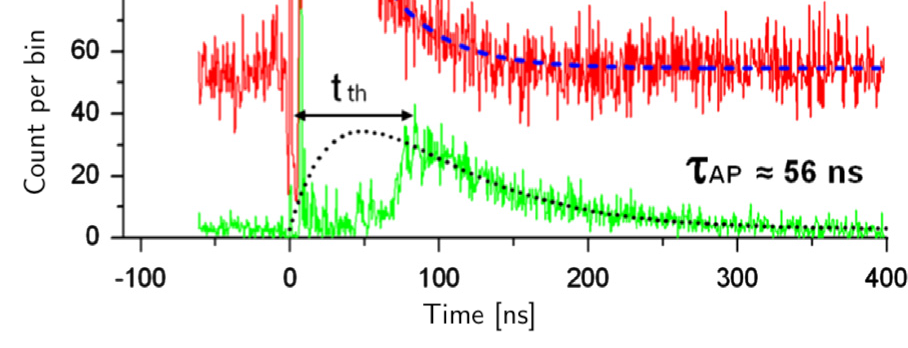
\includegraphics[width=\textwidth]{nagyap}
    
    \caption{\label{fig:nagyap} Excerpt of Figure~11 from \cite{nagy2014},
    showing the histogram of the delay of pulses successive to initial 1 PE
    pulses, selected with an upper bound on their amplitude to get afterpulses
    while removing dark count, and fitted with an exponential decay with
    constant $\tau_\text{AP}$ multiplied by the correction in
    \autoref{eq:recfactor} with $\tau_\text{rec} = \SI{207}{ns}$.}
    
\end{figure}

\cite{garutti2014} has approximately the same temporal cut and parameters, and
gets a good fit with either one or two uncorrected exponentials. We anticipate
that in our analysis the temporal cut will be even further relative to
$\tau_\text{rec}$ than in the referenced articles, so we will not be able to
discriminate the two models. For simplicity, we will keep the plain
exponentials.

The other matter with low delays is the amplitude reduction. Here all the
references we consulted agree on multiplying the 1 PE amplitude by the recharge
factor \eqref{eq:recfactor}, thus assuming that amplitude is proportional to
overvoltage. We will see this may not be accurate in our case.

Now to another topic: multiple afterpulses. The afterpulse avalanche itself
produces trapped carriers. However, since it may have smaller amplitude than a
primary avalanche, they will be less than those left around by a complete
discharge. Other two possible effects that we hypothesize, although we are not
sure about them, are: that if traps are not too far from saturation after an
avalanche, the additional afterpulses will be even more suppressed, and that an
avalanche may partially ``purge'' traps.

Keeping into account all these interactions is tedious, so we make a
simplifying assumption, inspired by the last consideration: that each avalanche
resets the cell to a fixed state. In this model, a pulse can have at most one
afterpulse. An eventual successive afterpulse must be produced by the first
afterpulse, not the initial pulse. \cite{cova1991} implicitly states that this
is not the case, although their experimental conditions are different because
the procedure they use to fill the traps is different from a ``spontaneous''
avalanche. Since these are second order effects, we anticipate that the
probabilities involved are small and that we probably would not be able to
falsify the simplified model with our data.

Bringing the DiCT model into the picture, each afterpulse will have its own
DiCT tree. We suppose that a smaller avalanche should emit less photons and
thus have less cross talk; again, for the sake of simplicity, we will assume
that the DiCT probability remains the same instead.

Since the DiCT involves separate cells, even with our ``resetting afterpulse''
model if the initial pulse has more than one PE then multiple afterpulses due
to the same initial pulse are allowed. We call this case \emph{parallel
afterpulses}, while the case with an afterpulse of an afterpulse \emph{series
afterpulses}.

\subsection{Expected values}
\label{sec:expval}

\cite[tab.~3.1~p.~62]{savarese2018} summarizes the noise parameters for the FBK
SiPMs at \SI{80}K and \SI{5}V overvoltage. In this analysis we will use newer
LFoundry SiPMs, so we can just get a rough idea from that. There are various
kinds of SiPM in the table, the low field near ultraviolet with medium
quenching resistance (last column) is the only one with the same recharge time
as ours ($\tau_\text{rec} = \SI{0.5}{\micro s}$) so we consider that values.
The dark count rate, converted from rate per area to rate per PDM (area
\SI{25}{cm^2}), is \SI{25}{cps}. The correlated noise probabilities are: DiCT
\SI{17}\%, AP \SI{17}\%, DeCT \SI{1.5}\%.

We did not make a model for DeCT (including delayed afterpulses) because we do
not have a clean selection of it in our data. In
\cite[fig.~3.8~p.~54]{savarese2018} we see that DeCT arrives within
\SI{50}{ns}. We will not properly analyze correlated pulses with delay below
\SI{100}{ns}. For the DeCT we will just give a very uncertain estimate. Since
the probability is smaller than the other noise modes, we completely neglect
second order effects due to DeCT.

\section{Data}

We use LNGS laser data for tile 21, produced by LFoundry. The LNGS data files
are:
%
\begin{verbatim}
LFOUNDRY/pre-production-test/TILE_21/LF_TILE21_77K_54V_65VoV_X.wav
LFOUNDRY/pre-production-test/TILE_21/LF_TILE21_77K_54V_69VoV_X.wav
LFOUNDRY/pre-production-test/TILE_21/LF_TILE21_77K_54V_73VoV_X.wav
\end{verbatim}
%
The `\texttt{X}' suffix in the file name stands for an index which goes from~1
to~10. Each file contains $\approx\num{20000}$ events, so we have \num{200000}
events per overvoltage.

The overvoltage is obtained by subtracting the first voltage from the second in
the file name and dividing by two. The first is the breakdown voltage while the
second is the applied reverse bias; the division is because the SiPM connection
layout in the PDM is parallel branches each with two SiPMs in series. Thus the
overvoltages are \SI{5.5}V, \SI{7.5}V, \SI{9.5}V.

We show the time-value histograms of a single file per overvoltage in
\autoref{fig:hist2dtile21}. These files do not include the laser trigger
waveform. Looking at the histograms it appears that the laser pulse arrives at
$\approx\SI{9}{\micro s}$ as usual. To be confident that we can assume the
trigger position, in \autoref{fig:triggerhist} we histogram all the triggers
from a lot of LNGS files. The full range of the distribution is
\SI[separate-uncertainty=true]{8969 \pm 11}{Sa}.

\begin{figure}
    
    \widecenter{\includempl{figtriggerhist}}
    
    \figcaption{triggerhist}{Cumulative histogram of the trigger leading edge
    (the first sample less than 600 in the recorded waveform) for 96 LNGS
    files. The distribution has the shape of a convolution between two uniforms
    with length 16 and~8, we suppose these are the clocks of the digitizer and
    laser triggers.}
    
\end{figure}

In some files there are double peaks in the fingerplot, i.e.~there are two
possible pulse amplitudes corresponding to the same number of PE. The worst
offender is the first file at \SI{5.5}{VoV},
\nolinkurl{LF_TILE21_77K_54V_65VoV_1.wav}. In \autoref{fig:doublepeak} we show
the fingerplot, both global and as a function of time, computed with
\SI{1.5}{\micro s} charge integration. It is evident that the pulse charge
changes during the acquisition. Since it is still possible to separate the PE
peaks, even if they are doubled, this will not be an issue. Moreover, with the
filter we will use in the analysis the doubling will be much less marked.

\begin{figure}
    
    \widecenter{\includempl{figdoublepeak}}
    
    \figcaption{doublepeak}{The distribution of the mean of the waveforms from
    sample 8958 to \num{10457} (1500 samples) in the first file at
    \SI{5.5}{VoV}. Left panel: global distribution. Right panel: the same
    distribution by groups of 200 events.}
    
\end{figure}

It was reported to us that in this data there could be a significative amount
of light that hits the detectors after being reflected. Since the apparatus is
small, we estimate an upper bound of \SI{1}m for the distance traveled by
light, which corresponds to a \SI{3}{ns} delay. This delay is smaller than
the scale of the variations of the signal shape and of the noise, so we can
neglect this problem.

\begin{figure}
    
    \widecenter{\includempl{fighist2dtile21-0}}

    \widecenter{\includempl{fighist2dtile21-1}}

    \widecenter{\includempl{fighist2dtile21-2}}
    
    \figcaption{hist2dtile21}{Time-value histograms of LFoundry tile~21 in LNGS
    laser data at overvoltages \SI{5.5}V, \SI{7.5}V, and~\SI{9.5}V.}
    
\end{figure}

\section{Peak finding}

As input to the analysis we will measure the amplitude and temporal position of
all the single pulses in the data. We will filter the waveforms to suppress
noise and then run a peak finding algorithm.

\subsection{Filtering}
\label{sec:filtering}

We filter each event using a cross correlation filter (see
\autoref{sec:filters}). We follow the procedure outlined in \autoref{ch:snr} to
make the filter template. We do the template separately for each file, to check
for unexpected variations in the pulse shape. The templates obtained are shown
in \autoref{fig:templates}. Although the variations appear to be reasonably
small, we use each template only for its own file.

\marginpar{Add more precise reference when I fix the template stuff.}

\begin{figure}
    
    \widecenter{\includempl{figtemplates}}
    
    \figcaption{templates}{Templates of the pulse shape obtained with averaging
    for each file.}
    
\end{figure}

An unexpected feature is the nonlinearity of the pulse amplitude with
overvoltage. A possible explanation is mislabeling of the overvoltages. The
overvoltage is determined from the bias and breakdown voltages reported in the
file name. The breakdown voltage is always the same because it is a property of
the tile, so if it was reported incorrectly, the correction to the overvoltage
would be a fixed offset. But in this case even if the ratio amplitude over
overvoltage would vary, the slope would be preserved, while in
\autoref{fig:templates} wee see that two equal overvoltage steps correspond to
clearly different absolute increases in amplitude.

One could think that the reported bias was incorrect, but it is a very simple
measurement. We will come back to this discussion after the analysis.

Filtering increases the signal to noise ratio, but degrades the separation
between close peaks. Since we are studying correlated pulses, it is thus
important to use a filter as short as possible. We filter the waveform with a
logarithmic range of filter lengths: \SI{32}{ns}, \SI{64}{ns}, \ldots,
\SI{2048}{ns}. The computations we will describe are carried in parallel with
all filter lengths, and then we choose in the analysis which lengths to use.
The truncation of the template to the desired length is done like in
\autoref{ch:timeres}, keeping the fixed length subrange of samples that has
maximum squared norm.

\marginpar{When I fix the template stuff, the chapter for the truncation will
be \autoref{ch:snr}.}

As usual the template is normalized to unit sum for filtering, such that the
filter behaves like an average and the baseline can be computed independently
of the filter. This also means that signals will stay negative.

To evaluate the filter near the boundaries, the waveform is prolonged with the
estimated baseline value, described in the next section. We defer to
\autoref{sec:pe} the description of how we select the filter length.

\subsection{Baseline}

To compute the height of the peaks we have to subtract the baseline value. We
compute the baseline using the pre-trigger region of the waveforms. For
robustness against deviations we use the median instead of the average. The ADC
has relatively low resolution (10~bit), so since the median can output only one
of the values of the input sequence it is quantized. To have a more continuous
output we divide the array in 8 interleaved subarrays, i.e.\ the first subarray
contains samples 0, 8, 16, \dots, the second 1, 9, 17, etc., take the median
separately on each subarray, and then average the medians.

If any pre-trigger sample in an event is less than 700, for that event we reuse
the baseline obtained in a previous event.

In \autoref{fig:baseline} we show the histogram of the obtained baseline values
for the \SI{5.5}{VoV} data. We will carry on the discussion always on the
\SI{5.5}{VoV} dataset as example, unless otherwise necessary.
Appendix~\ref{ch:analplot} contains additional plots that complete the picture.

\begin{figure}
    
    \widecenter{\includempl{figbaseline}}
    
    \figcaption{baseline}{Distribution of the waveform baseline measured in
    the pre-trigger region of the events. See \autoref{fig:baseline2} for all
    overvoltages.}
    
\end{figure}

The baseline distribution has a small tail to the left (note that the scale is
logarithmic) and some far outliers. In \autoref{fig:bsoutlier} and
\autoref{fig:bstail} we show the events corresponding to the lowest and highest
measured baselines and a pair of events from the lower tail respectively. (The
event visualization contains elements which we have not introduced yet, they
will soon be explained.)

\begin{figure}
    
    \widecenter{\includempl{figbsoutlier-0}\includempl{figbsoutlier-1}}

    \figcaption{bsoutlier}{The events with the lowest and highest baseline.
    See \autoref{fig:bsoutlier2} for all overvoltages.}

\end{figure}

\begin{figure}
    
    \widecenter{\includempl{figbstail-0}\includempl{figbstail-1}}

    \figcaption{bstail}{A pair of events from the low baseline tail (baseline
    between 955 and 956). See \autoref{fig:bstail2} for all overvoltages.}

\end{figure}

In all cases the extreme baseline events do not show anomalies, they have
genuinely unusual baselines. At \SI{5.5}{VoV} and \SI{9.5}{VoV} the events
corresponding to the lowest and highest baseline have close progressive
indices, so they must occur close in time; we suppose then that these
deviations are due to low-frequency transient oscillations.

The events in the tail all have a pre-trigger pulse (we checked only the two
ones we plotted, we did not handpick). This means that we will systematically
underestimate the amplitude of pre-trigger pulses. However, as is already
evident by looking at the event plots, the bias is small compared to the pulse
height. If data with lower SNR was to be processed, we would up the baseline
veto value from 700 to something as close as possible to the noise pedestal and
segment the baseline computation to detect inhomogeneity, but in our present
case we will go on without fixing this bias.

\subsection{Laser peak}
\label{sec:laser}

We know where the laser pulse should be, so we search it separately from other
pulses. We take a window from the filtered waveform of \SI{\pm 30} samples
around the expected trigger position 8969. In this window we take the minimum
local minimum, i.e.\ we consider the samples which have higher neighboring
samples, and take the minimum of these. If there is no local minimum, which
happens when the waveform is monotonically increasing or decreasing within the
60 selected samples, we mark the laser peak as missing.

To check that this is working we look at the distribution of the peak positions
for 1 PE pulses (\autoref{fig:laserpos}, left panel). It is centered on 8969 as
expected. However, it has a tail to the right when the filter length is short.
An explanation that comes to mind is that maybe when the SNR is not high
enough, the peak finder is picking up a close afterpulse instead of the main
peak. Given the short delay this should be unlikely, but since we are
particularly interested in afterpulses it is better to check this thoroughly.

\begin{figure}

    \widecenter{\includempl{figlaserpos-0}\includempl{figlaserpos-1}}

    \figcaption{laserpos}{Left panel: histogram of the laser peak position,
    only for 1 PE peaks, for all filter lengths. The zero of the scale is such
    that the expected position is 8969. Right panel: 2D histogram of the laser
    peak position and the amplitude, for the same selection of peaks, but only
    with the \SI{128}{ns} filter. See \autoref{fig:laserpos2} for all
    overvoltages.}
    
\end{figure}

As a first diagnostic, we look at the joint distribution of the peak position
and height (\autoref{fig:laserpos}, right panel). If the minimum was moving to
the right due to an additional close peak, we would expect a positive
correlation between height and position in the tail. Instead, we see a negative
correlation.

Then we look at the events themselves. In \autoref{fig:lptail} we show the
event with the rightmost position at \SI{64}{ns}, filtered with \SI{64}{ns} and
\SI{128}{ns}. With the longer filter the position goes back to the center of
the distribution. We inspected a lot of events in the tail and they are almost
all like the one we show.

\begin{figure}

    \widecenter{\includempl{figlptail-0}\includempl{figlptail-1}}

    \figcaption{lptail}{Left panel: the event with the rightmost laser peak
    position for 1 PE peaks with filter length \SI{64}{ns}. Right panel: the
    same event with filter length \SI{128}{ns}. See \autoref{fig:lptail2} for
    all overvoltages.}

\end{figure}

Finally, the tail contracts as the overvoltage increases (see
\autoref{fig:laserpos2}). From these observations we induce that the right
shift is caused by random fluctuation. The asymmetry of the tail reflects the
asymmetry of the shape of the signal.

We have not said how we are selecting 1 PE pulses. The explanation will come in
\autoref{sec:pe}. Also, we have talked about the positions of the peaks in the
filtered waveform without specifying the alignment of the filter output
relative to the input. For example, in the histogram (\autoref{fig:laserpos})
the position is centered on the assumed trigger 8969, while clearly in the
event visualization (\autoref{fig:lptail}) the peak search range is after the
trigger. The reader has to trust us that although we employ multiple
conventions, we use them consistently each time.

We said that with our procedure a laser peak can be missing. However we know
that the laser is always present; even when there are no pulses, we need to
count the event as a 0 PE laser signal to fit the Poisson+DiCT distributions.
We have to make something of the ``missing laser'' events.

First, we count these events for each filter length (\autoref{fig:missing},
left panel). They are about \SI{1.5}\% of the total, so not negligible. We went
through a lot of these events and they are almost all genuinely missing pulses.
It turns out that the noise is actually quite likely not to produce a local
minimum in a \SI{60}{ns} window after filtering. Nevertheless, there are some
events which have a pulse which for some weird combination of noise
oscillations is not detected properly.

\begin{figure}

    \widecenter{\includempl{figmissing}}
    
    \figcaption{missing}{Left panel: for each overvoltage, the fraction of
    events where there is no local minimum in the laser peak search range, as a
    function of filter length. Right panel: the fraction of events where the
    minimum is missing for all filter lengths less than or equal to the one on
    the abscissa.}

\end{figure}

As in the case of the right shift, the anomalies tend to appear only for a
particular filter length choice and disappear on the same event with other
lengths. So as a simple solution we use the shortest filter which yields a
non-missing peak when the preferred filter does not work. The right panel of
\autoref{fig:missing} shows how the fraction of missing events decreases as we
allow more lengths to choose from. Even with this fix, however, there is a hard
core of events which do not have a local minimum in any case; from \SI{0.03}\%
at \SI{5.5}{VoV} to \SI{0.15}\% at \SI{9.5}{VoV}.

These events are more interesting, so we show 12 of them at random for each
overvoltage in Figures~\ref{fig:verymissing0}, \ref{fig:verymissing1},
and~\ref{fig:verymissing2}. With our good old eyes, we identify three cases:
1)~true missing pulses, 2)~delayed pulses which fall out of the window, and
3)~pulses which are shadowed by a very high close consecutive pulse. In
\autoref{tab:missing} we list the total number of hard misses and the counts
of the three categories in the sample for all overvoltages.

\begin{table}
    
    \widecenter{
        \begin{tabular}{S[table-format=1.1] S[table-format=3] *3S[table-format=1]}
            \toprule
            & & \multicolumn3c{Count of 12} \\
            \cmidrule(r){3-5}
            {Overvoltage [\si{V}]} & {Total} & {True miss} & {Delayed} & {Close consecutive} \\
            \midrule
            5.5 &  56 & 4 & 3 & 5 \\
            7.5 & 148 & 7 & 5 & 0 \\
            9.5 & 303 & 5 & 0 & 7 \\
            \bottomrule
        \end{tabular}
    }
    
    \tabcaption{missing}{The number of events where the laser peak is missing
    with all filter lengths, and the counts, in a random sample of 12 of these
    events, for the three categories of configurations that appear in this
    selection.}
    
\end{table}

The delayed pulses could be photons that produce carriers in an inactive region
that then migrate to a diode junction (we are not sure about this, it is just
speculation). The consecutive pulses could be DeCT with high DiCT, they would
have the time scale we expect from \cite[fig.~3.8~p.~54]{savarese2018}
already mentioned in \autoref{sec:expval}, or less likely afterpulses.

Since these events are a small fraction of the sample we did not fix this
further. We will just keep in the back of our minds that there are these events
and check case by case that ignoring them has a negligible effect.

\subsection{Other peaks}

We identify other pulses using a prominence-based peak finder. With
``prominence'' we mean the topographical prominence, which is defined as
follows: starting from the peak whose prominence is to be measured, go to the
right and to the left until an higher elevation is found. For each side, take
the minima between these stops and the peak. The prominence is the difference
in elevation between the peak and the maximum of the two minima. See
\autoref{fig:prominence} for an illustration.

In this discussion we will use positive signal logic, so a peak is a local
maximum. Remember that in the actual analysis the convention is swapped.

\begin{figure}
    
    \widecenter{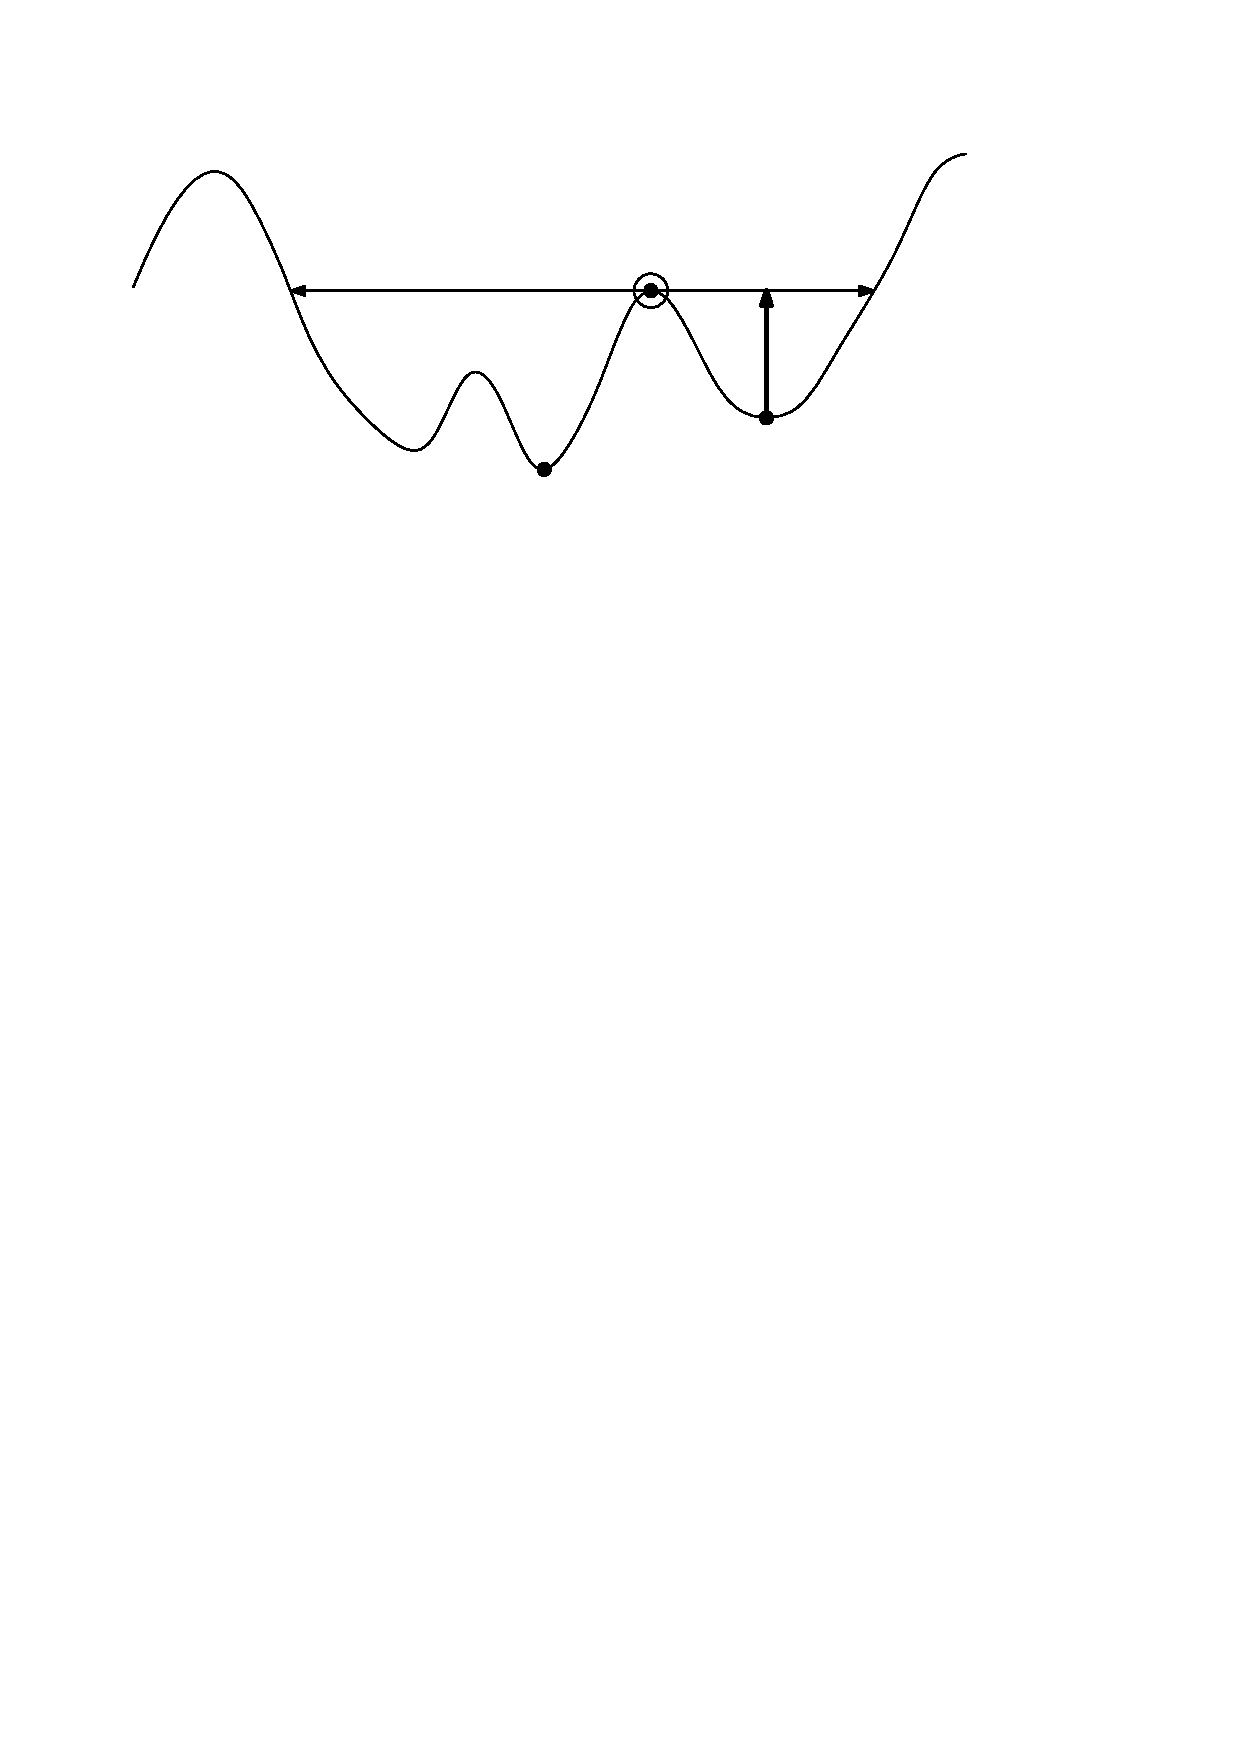
\includegraphics[width=0.8\textwidth]{prominence}}
    
    \caption{\label{fig:prominence} Illustration of the definition of
    topographical prominence. The prominence of the circled peak is the length
    of the thick vertical arrow.}
    
\end{figure}

We search the peaks separately in the pre and post laser peak regions. When the
laser peak is missing, we use the beginning of the laser peak search range as
separator. This means that even if the laser peak is lower than the peak, the
prominence ``exploration range'' stops there.

If one of the minima occurs at the edge, it is ignored and the prominence is
computed using the minimum on the other side, unless both minima occur at the
edge. This is to avoid assigning a very low prominence to a pulse whose shape
is truncated due to being close to a boundary.

The minima are capped to the baseline: if a minimum is lower than the baseline,
the value of the baseline is used instead to compute the prominence. This
increases the ratio between the prominence of close pulses to the one of
isolated pulses, because if the explored range is longer it is easier to find a
deeper random oscillation.

For each region, we save the two most prominent peaks. We do not make a
selection on the prominence, we always fill the four slots per event. In this
way we can observe the distribution of the height of random peaks and choose
a good threshold afterwards.

In peak finding algorithms it is customary to require a minimum distance
between peaks. This is to avoid picking up close high peaks due to random
oscillation that actually correspond to a single pulse. Selecting by prominence
avoids this problem if the waveform is smooth, because close peaks will have a
shallow dip between them and the prominence of the lower one will be measured
relative to that. Our waveforms are smooth on the scale of the filter length,
so it did not turn out necessary to add a distance criterion.

In \autoref{fig:peakfinder} we show two examples of events with close
afterpulses correctly identified.

\begin{figure}
    
    \widecenter{\includempl{figpeakfinder-0}\includempl{figpeakfinder-1}}
    
    \figcaption{peakfinder}{The events with the closest pair of pre-trigger
    pulses (left panel) and post-trigger pulse closest to the laser pulse
    (right panel) for at least 1 PE peaks.}
    
\end{figure}

\subsection{PE}
\label{sec:pe}

To assign the number of PE to the peaks we need to define bins for the height
of the peaks. We want to choose the filter length that yields the optimal
separation between PE in the height distribution. A longer filter suppresses
the random height fluctuation due to noise; at the same time, however, it picks
up afterpulses with the template tail, adding an upper tail to each PE height
distribution. Since the afterpulse probability increases with the number of PE
of the primary pulse, the distributions for 0 and 1~PE are the least touched.

In our analysis we will care particularly about selecting 1~PE pulses and
separating the afterpulses. So we use the following criterion: we take the
shortest filter that allows to clearly separate the 1~PE distribution. These
filter lengths are respectively \SI{128}{ns}, \SI{64}{ns}, \SI{64}{ns} for
\SI{5.5}{VoV}, \SI{7.5}{VoV}, \SI{9.5}{VoV}. We show the templates for these
lengths in \autoref{fig:trunc}.

\begin{figure}

    \widecenter{\includempl{figtrunc}}
    
    \figcaption{trunc}{The principal filter templates used in the analysis,
    shown unnormalized.}
    
\end{figure}

We tried selecting away the afterpulse tails using the peak finder to locate
afterpulses, however we did not manage to reduce them significantly. We
interpret this as the tail being composed mainly of close and short
afterpulses, that can not be recognized individually due to their low height.
Being located on the slope of the laser peak, the prominence of a close
afterpulse tends to be lower that that of an isolated pulse with the same
height. Thus the peak finder will always find two random peaks in the noise
with higher prominence than a short afterpulse, forbidding us to try to use an
aggressively low threshold with an high fake rate, since those afterpulses are
not even present in the peaks list.

There are other two minor factors that deform the height distribution: the
saturation of the digitizer, and pre-trigger pulses close to the laser one.
Thus we histogram the laser peak height excluding events with saturation and
events where the peak finder locates a pre-trigger pulse higher than~8 within
\SI{2.5}{\micro s} before the trigger using the longest filter. This
histogram is shown in \autoref{fig:pe} for \SI{5.5}{VoV} and \autoref{fig:pe2}
for all overvoltages.

\begin{figure}
    
    \widecenter{\includempl{figpe}}
    
    \figcaption{pe}{Histogram of the laser peak height, with a selection to
    avoid biased heights. The dotted lines are the boundaries of the PE bins.
    See \autoref{fig:pe2} for all overvoltages.}
    
\end{figure}

We place the PE bin boundaries taking the midpoints between the two most
distant consecutive heights in the range between each pair of consecutive
height distribution peaks. Heights above the last boundaries are not assigned a
number of PE, but they are not lost for the analysis, we will just use an
overflow bin when necessary. The ruler ticks that accompany the peaks in the
event visualizations are these boundaries.

Note the dips between the peaks in the histograms (the vertical scale is
logarithmic). The lowest bin count is at most~4 in all cases. Let us put a
rough upper bound on the contamination. There are more than \num{10000} events
per peak. Supposing a worst case with 25 bins with 4 counts each penetrating
into a neighboring peak, it gives \SI1\%. This means that it is surely less
than the Poisson error on the count for each PE. The 1~PE peaks are well
separated, with a row of 0 or 1~count bins around them, so we estimate a
contamination of \SI{0.01}\%.

\subsection{Amplitude of close pulses}

When two pulses are close to each other, the height contains a contribution
from the tail of the other pulse. We need to compute the amplitude of the
single pulse, i.e.\ the height it would have if it was isolated. To simplify
the problem, we make the following assumptions:
%
\begin{enumerate}
    
    \item the position of a peak does not depend on the presence of other
    pulses;
    
    \item the shape of afterpulses is the same as normal pulses.
    
\end{enumerate}

About the first assumption: we have seen that the peaks in the output of the
cross correlation filter have a sharp cusp. A perfectly sharp cusp, even if
summed to a sloping shape, remains in the same position. A rounded peak,
instead, will move slightly in the uphill direction when summed to a slope.
Actually, given the short filters we are using, these cusps are not really
sharp. Look at the second panel of \autoref{fig:peakfinder}. The peak in the
square box has a radius of less than \SI{10}{ns}. By intuition we expect the
peak to drift less than its radius, so we estimate that the typical error will
be \SI{5}{ns}.

About the second assumption: it seems that in the literature this is implicitly
given for. But, as we said before, it depends on the assumption that the pulse
shape does not change with overvoltage, such that while the cell is recharging,
its behavior will just be the rescaled version of its fully charged self. In
\autoref{sec:filtering} we have seen that the pulse amplitude does not depend
linearly on overvoltage. If you look closely at \autoref{fig:templates}, you
can notice that the shapes are also a bit different. We make a clearer
comparison in \autoref{fig:shape} by plotting the templates normalized to have
the same peak amplitude. They are indeed different, but the difference is small
enough to justify the working hypothesis.

\begin{figure}
    
    \widecenter{\includempl{figshape}}

    \figcaption{shape}{The signal templates at different overvoltages compared
    fixing the peak amplitude to~1. The thickness of the stroke is twice the
    standard deviation over the 10 files per overvoltage, while the center of
    the stroke is the mean.}
    
\end{figure}

Now, let $\mathbf y$ be the output of the filter applied to a single noiseless
pulse, which we compute by filtering the signal template. Let $t_\alpha$ be the
position of peak $\alpha$ and $a_\alpha$ the unknown amplitude. Since the
filter is linear, the filtered sum of the pulses and the noise is the sum of
each component filtered separately, so the model for the complete filtered
waveform $\mathbf w$ is
%
\begin{equation}
    w_i = \sum_\alpha a_\alpha y_{i - t_\alpha} + \epsilon_i,
\end{equation}
%
where $\boldsymbol\epsilon$ is the filtered noise. There is some freedom in the
definition of $\mathbf y$: we fix that the peak occurs at $y_0$ and that $y_0 =
1$, such that if there is only one peak then $w_{t_1} = a_1 + \epsilon_{t_1}$.

It is well known that the minimum variance in estimating $\mathbf a$ is
obtained by using least squares with the inverse of the covariance matrix $V$
of $\boldsymbol\epsilon$ as quadratic form. Let $H_{i\alpha} = y_{i-t_\alpha}$,
then the solution is \cite[628]{zyla2020}
%
\begin{equation}
    \hat{\mathbf a} = (H^\top V^{-1} H)^{-1} H^T V^{-1} \mathbf w.
    \label{eq:lsq}
\end{equation}
%
We note, however, that to solve the system it is just necessary to have as many
datapoints as the number of peaks. It then comes natural to solve for
simplicity this system of equations instead:
%
\begin{equation}
    w_{t_\beta} = \sum_\alpha \hat a_\alpha y_{t_\beta - t_\alpha},
    \label{eq:amplsystem}
\end{equation}
%
i.e.\ we use only the observed peak heights $w_{t_\beta}$ instead of the full
waveform.

What are we losing with this simplification? In \autoref{sec:filters} we said
that the matched filter is equivalent to linear least squares. We now indeed
show that, if we were using the matched filter, solving \eqref{eq:amplsystem}
would be equivalent to least squares and thus optimal. Just for this proof, let
us use all the above notation, but without the filter applied, i.e.\ $\mathbf
w$ is the unfiltered waveform, $\mathbf y$ is the unfiltered signal, $V$ is the
covariance of the unfiltered noise.

The template of the matched filter is
%
\begin{equation}
    \mathbf h = V^{-1} \mathbf y.
\end{equation}
%
The model (noise implicit) is
%
\begin{equation}
    \mathbf w = H \mathbf a.
\end{equation}
%
The filter is applied by operating with the matrix
\begin{equation}
    F_{ij} \equiv h_{j-i} = V^{-1}_{j-i,k} y_k,
\end{equation}
%
so applying the filter we have
%
\begin{align}
    F \mathbf w &= F H \mathbf a. \label{eq:noindices}
\end{align}
%
We want to use only the peak heights in the filter output, assuming that we
know exactly the true signal positions. These are
%
\begin{equation}
    W_\beta \equiv (F \mathbf w)_{t_\beta} = V^{-1}_{j-t_\beta,k} y_k w_j. 
\end{equation}
%
The noise is stationary, so we can sum the same offset to the indices of
$V^{-1}$. Using this fact, the symmetry of $V$, and redefining the mute index
$k$, we obtain

\marginpar{This translation of the indices of $V^{-1}$ holds only in the limit
of an infinitely long waveform. In practice for a waveform with some margin
around the pulses.}

\begin{equation}
    W_\beta = V^{-1}_{jk} y_{k-t_\beta} w_j = V^{-1}_{jk} H_{k\beta} w_j
    \rightarrow \mathbf W = H^\top V^{-1} \mathbf w.
\end{equation}
%
So, considering only the $W_\beta$ on the left hand side of
\eqref{eq:noindices} and putting the indices on the right hand side, we have
%
\begin{align}
    W_\beta &= V^{-1}_{j-t_\beta,k} y_k H_{j\alpha} a_\alpha = \\
    &= V^{-1}_{j,k} y_{k-t_\beta} H_{j\alpha} a_\alpha = \\
    &= (H^\top V^{-1} H)_{\beta\alpha} a_\alpha,
\end{align}
%
thus the solution is
%
\begin{equation}
    \mathbf a = (H^\top V^{-1} H)^{-1} H^\top V^{-1} \mathbf w,
\end{equation}
%
which is the least squares estimator \eqref{eq:lsq}. \hfill $\square$

Our filter differs in two ways from the matched filter: it does not keep into
account the noise correlation, and it is truncated. So our method for computing
the amplitude is worse than the optimal one as much as the filter is worse than
the matched filter.

In each event we have to decide which peaks to input in \eqref{eq:amplsystem}.
Most of the time, peaks are random noise oscillation. If the amplitude of
random peaks had mean zero, adding a fake peak would increase the error but not
introduce a bias. But, since we are selecting peaks by highest prominence, it
is guaranteed that in a region of some microseconds we will find a peak with
height comparable to the noise standard deviation. Indeed in the next section
we will look at the height distribution for the peak finder output and see that
it is positively biased. So we compute the amplitude only for peaks higher than
a threshold. As threshold we pick the the PE bin boundary between 0 and 1~PE.

When we use the computed pulse amplitude instead of the peak height, we would
like to also see the distribution of the fake peaks such that we can be sure at
a glance that we have no contamination, but most of the fake peaks do not have
an amplitude since they do not pass the threshold prerequisite. The $y$
normalization we have chosen makes the amplitude ``have the same units'' of the
height, so we construct a variable which is the amplitude when available, and
the height otherwise. In the following sections we mean this variable when we
talk about ``amplitude''.

Note that with this selection we are not excluding short afterpulses from the
amplitude computation, because even if their amplitude is smaller, sitting on
the tail of their parent pulse their height is still above threshold.

In the event visualizations, the ruler associated to each peak starts from a
dot placed such that the distance from the dot to the peak is the amplitude.
In the legend, the amplitude is given under ``$a = \ldots$''.

\section{Random pulses rate}

When counting afterpulses there will be a background from the dark count rate,
which we have to subtract, so we measure it in the pre-trigger region. The
laser trigger frequency should be less than \SI{1}{kHz}, so the events are
distant between each other and there is not the possibility of correlated noise
from a laser pulse leaking into the successive event.

\marginpar{What is the laser trigger rate? Specify this better if I know after
writing \autoref{ch:data}.}

The title of this section reads ``random pulses rate'' instead of dark count
rate because we will see we have reason to believe that in the data there are
actually more random pulses than the dark count. It does not matter for
background subtraction though.

By looking at the time-value histograms in \autoref{fig:hist2dtile21} we see
that in \num{20000} events there are just a few pre-trigger pulses, so we
neglect the case of a double random pulse in the same event. If there are two
pre-trigger pulses, one must be the afterpulse of the other, so the event
counts as one random pulse. For the rate we do not care to know which pulse is
the primary, but we will need it when fitting the DiCT model to the random
pulses.

The primary pulse is of course the first in chronological order, but to
distinguish the one pulse from the two pulses case we are forced to put a
threshold on the amplitude before looking at the distribution. We do something
similar as we did for the amplitude. The initial variables are the position,
height and amplitude of the two most prominent pre-trigger peaks. When both
heights are above the 0 to 1~PE boundary, the first set of variables is set to
the first peak in chronological order; otherwise to the most prominent peak.

In the left panel of \autoref{fig:pretrigger} we show the scatter plot of the
first pulse amplitude versus position. There are some problems at the edges. On
the left edge, the negative amplitudes are actually very large values that we
mapped to \num{-10}. They are probably due to the amplitude linear system
\eqref{eq:amplsystem} being degenerate, but we did not investigate why this may
happen. On the right edge conversely there are some zeroes and anomalously
small values. Thus we ignore the first \SI{100}{ns} and the last \SI{500}{ns}
of the pre-trigger region. The wider margin on the right is just to be safe in
case the presence of the laser pulse was having some effects. The selected
region is marked by the gray vertical band in the plot.

\begin{figure}
    
    \widecenter{\includempl{figpretrigger-0}\includempl{figpretrigger-1}}
    
    \figcaption{pretrigger}{Left panel: scatter plot amplitude vs.\ position of
    the chronological first pre-trigger peak in each event. Right panel:
    histogram of the amplitude for the peaks contained in the vertical gray
    band in the left plot. See \autoref{fig:pretrigger2} for all overvoltages.}
    
\end{figure}

The right panel of \autoref{fig:pretrigger} shows the histogram of the
amplitude of the pulses in the temporal cut. The separation between random
peaks and 1~PE pulses is clear; the amplitude threshold we use is marked with a
gray band also reported in the left panel. The dotted lines are the PE bin
boundaries. As we anticipated, the distribution of the amplitude of the random
peaks is biased upward, and leaks a bit above the 0 to 1~PE boundary.

To compute the rate, we count the number of pulses satisfying the cuts, and
divide by the number of events times the pre-trigger region duration minus the
cuts. The uncertainty is given by the Poisson error of the count. In
\autoref{tab:ptrate} we report the obtained values.

\begin{table}
    
    \widecenter{
        \raisebox{-0.5\height}{\includempl{figptrate}}
        \begin{tabular}{
            S[table-format=1.1]
            S[table-format=6]
            S[table-format=1.2]
            S[table-format=1.2]
            S[table-format=3]
            S[table-format=3(2), separate-uncertainty=true]
        }
            \toprule
            &
            & \multicolumn2c{Time}
            & \multicolumn2c{Pulses} \\
            \cmidrule(r){3-4} \cmidrule(r){5-6}
            {Overvoltage}
            & {Events}
            & {Per event}
            & {Total}
            & {Count}
            & {Rate} \\
            {[\si V]}
            &
            & {[\si{\micro s}]}
            & {[\si s]}
            &
            & {[\si{cps}]} \\
            \midrule
            5.5 & 200028 & 8.37 & 1.67 &  73 &   44 \pm 5 \\
            7.5 & 200021 & 8.37 & 1.67 & 277 & 165 \pm 10 \\
            9.5 & 200025 & 8.37 & 1.67 & 186 &  111 \pm 8 \\
            \bottomrule
        \end{tabular}
    }
    
    \tabcaption{ptrate}{The rate of primary pre-trigger pulses in a fiducial
    region and the intermediate quantities used to compute it.}
    
\end{table}

We notice that the rate at \SI{7.5}{VoV} is substantially higher than the one
at \SI{9.5}{VoV}. The dark count rate steadily increases with overvoltage (see
for example \cite[fig.~3.13~p.~61]{savarese2018}), because an higher field in
the diode lowers the potential barrier that a carrier must overcome to become
conducive. So we induce that there must be an additional source of random
pulses. Maybe the experimental setup was not light-tight. Anyway, these values
can be considered an upper bound for the dark count rate. For reference, the
maximum dark count rate allowed by the DarkSide20k specifications is
\SI{250}{cps} \cite[tab.~3.1~p.~62]{savarese2018}.

\section{Afterpulses}

% dire come li seleziono (anche che prendo il primo a sinistra)
% come calcolo l'ampiezza, questione di quando non è definita
% spiegare la questione del "primo venuto"

\begin{figure}
    
    \widecenter{\includempl{figapampl-0}\includempl{figapampl-1}}

    \widecenter{\includempl{figapampl-2}\includempl{figapampl-3}}
    
    \figcaption{apampl}{}
    
\end{figure}

\begin{figure}
    
    \widecenter{\includempl{figapscatter-0}\includempl{figapscatter-1}}

    \figcaption{apscatter}{See \autoref{fig:apscatter2} for all overvoltages.}
    
\end{figure}

\begin{figure}
    
    \widecenter{\includempl{figapfit-0}\includempl{figapfit-1}}

    \figcaption{apfit}{See \autoref{fig:apfit2} for all overvoltages.}
    
\end{figure}

\begin{table}
    
    \widecenter{
        \scriptsize\sffamily
        \setlength\tabcolsep{4pt}
        \begin{tabular}{
            S[table-format=1.1]
            S[table-format=3]
            S[table-format=4]
            S[table-format=5]
            S[table-format=3]
            S[table-format=1.2]
            S[table-format=2.1(2)]
            S[table-format=2.1(2)]
            S[table-format=3(2)]
            S[table-format=1.2(2)]
            S[table-format=2.1(2)]
            S[table-format=1.3(2)]
            S[table-format=1.2(2)]
            S[table-format=2]
            S[table-format=2]
            S[table-format=1.2]
        }
            \toprule

            & \multicolumn2c{Delay cut}
            & {}
            & {}
            & {}
            & {}
            & \multicolumn4c{Fit parameters}
            & {}
            & {}
            & \multicolumn3c{Fit quality} \\
            \cmidrule(r){2-3} \cmidrule(r){8-11} \cmidrule(r){14-16}
            {OV}
            & {From}
            & {To}
            & {Events}
            & {Cnt}
            & {Time}
            & {Random}
            & {Random}
            & {tau1}
            & {tau2}
            & {p1}
            & {Correction}
            & {Prob.}
            & {chi2}
            & {dof}
            & {pval} \\
            {[\si V]}
            & {[\si{ns}]}
            & {[\si{ns}]}
            &
            &
            & {[\si s]}
            &
            &
            & {[\si{ns}]}
            & {[\si{\micro s}]}
            & {[\si\%]}
            &
            & {[\si\%]}
            &
            &
            & \\
            \midrule
5.5 & 300 & 5500 & 46990 & 535 & 0.24 & 10.7 \pm 1.2 & 11.6 \pm 1.2 & 399 \pm 19 &        {n.d.} &       {n.d.} &   2.12 \pm 0.16 & 2.37 \pm 0.21 & 77 & 17 & {<1e-6} \\
5.5 & 300 & 5500 & 46990 & 535 & 0.24 & 10.7 \pm 1.2 & 10.7 \pm 1.2 & 285 \pm 27 & 2.24 \pm 0.64 & 71.9 \pm 4.2 & 2.116 \pm 0.084 & 2.36 \pm 0.14 & 22 & 17 &     0.17 \\ \midrule
7.5 & 300 & 5500 & 38404 & 590 & 0.20 & 33.0 \pm 2.0 & 35.1 \pm 1.9 & 432 \pm 22 &        {n.d.} &       {n.d.} &   2.00 \pm 0.14 & 2.91 \pm 0.24 & 75 & 18 & {<1e-6} \\
7.5 & 300 & 5500 & 38404 & 590 & 0.20 & 33.0 \pm 2.0 & 33.2 \pm 2.0 & 283 \pm 30 & 2.04 \pm 0.59 & 68.5 \pm 4.9 & 2.049 \pm 0.080 & 2.97 \pm 0.17 & 20 & 18 &     0.31 \\ \midrule
9.5 & 300 & 5500 & 28301 & 605 & 0.15 & 16.4 \pm 1.2 & 17.0 \pm 1.2 & 537 \pm 27 &        {n.d.} &       {n.d.} & 1.749 \pm 0.096 & 3.64 \pm 0.25 & 69 & 18 & {<1e-6} \\
9.5 & 300 & 5500 & 28301 & 605 & 0.15 & 16.4 \pm 1.2 & 16.3 \pm 1.2 & 227 \pm 38 & 1.13 \pm 0.15 & 47.7 \pm 7.6 & 1.908 \pm 0.068 & 3.97 \pm 0.22 & 11 & 18 &     0.91
            \\ \bottomrule
        \end{tabular}
    }
    
    \scriptcaption{tab}{tab}{ap}{}
    
\end{table}

\begin{figure}
    
    \widecenter{\includempl{figapresults}}

    \figcaption{apresults}{}

\end{figure}

\section{Delayed cross talk}

\begin{figure}
    
    \widecenter{\includempl{figdect}}
    
    \figcaption{dect}{}
    
\end{figure}

\section{Direct cross talk}

\subsection{Random pulses}

\subsection{Afterpulses}

\subsection{Laser pulses}

\subsection{Results}

\section{Conclusions}

% VETO
% simulazione (confronto con cosa c'è in Pyreco, dire che è quasi il nostro
% stesso modello)
% dire che i casini per delay piccoli con gli afterpulse alla fine non
% dovrebbero contare troppo perché l'ampiezza è più piccola
% scusarsi per non aver fatto gli ovvi miglioramenti: fittare con più di 1 pe
% come selezione iniziale per gli afterpulse, modellare meglio l'altezza degli
% afterpulse, studiare un modello empirico intermedio per il cross talk,
% tenere conto dei doppi picchi nei fit.
% peak finding, citare LZ:
% Conferenza dance machine learning workshop
% https://indico.physics.lbl.gov/event/1192/contributions/4934/

% cosa che si può migliorare: usare il filtro lungo quando calcolo l'ampiezza.
% ma questo sta già nella discussione di LZ.
